\newpage
\changefontsizes{16pt}
\centerline{\textbf{CHƯƠNG II: MỘT SỐ ỨNG DỤNG THỰC TẾ}}

\vspace{1cm}
\changefontsizes{15pt}
\setlength{\parindent}{0cm}
\textbf{Dự đoán mức tăng trưởng của một loại cổ phiếu}

\vspace{0.5cm}
\changefontsizes{13pt}
\setlength{\parindent}{0cm}


Đây mà một lĩnh vực mà không phải ai cũng am hiểu, không phải ai cũng thích hợp để tham gia vào. Nó đòi hỏi không chỉ tài năng nghiên cứu thị trường của người chơi cổ phiếu mà còn là những hành động quyết đoán dựa trên các tính toán của mình.

\bigskip
Để có thể dự đoán được giá trị của cổ phiếu trong khoảng thời gian nào đó sắp tới, người đầu tư chuyên nghiệp cần phải điều tra vô số các yếu tố về thị trường, chính trị, xã hội,... các yếu tố này sẽ ảnh hưởng trực tiếp đến giá của cổ phiếu. Tuy nhiên các yếu tố vừa kể không hề đơn giản để thu thập và tính toán.




\begin{center}
	\begin{figure}[htp]
		\begin{center}
			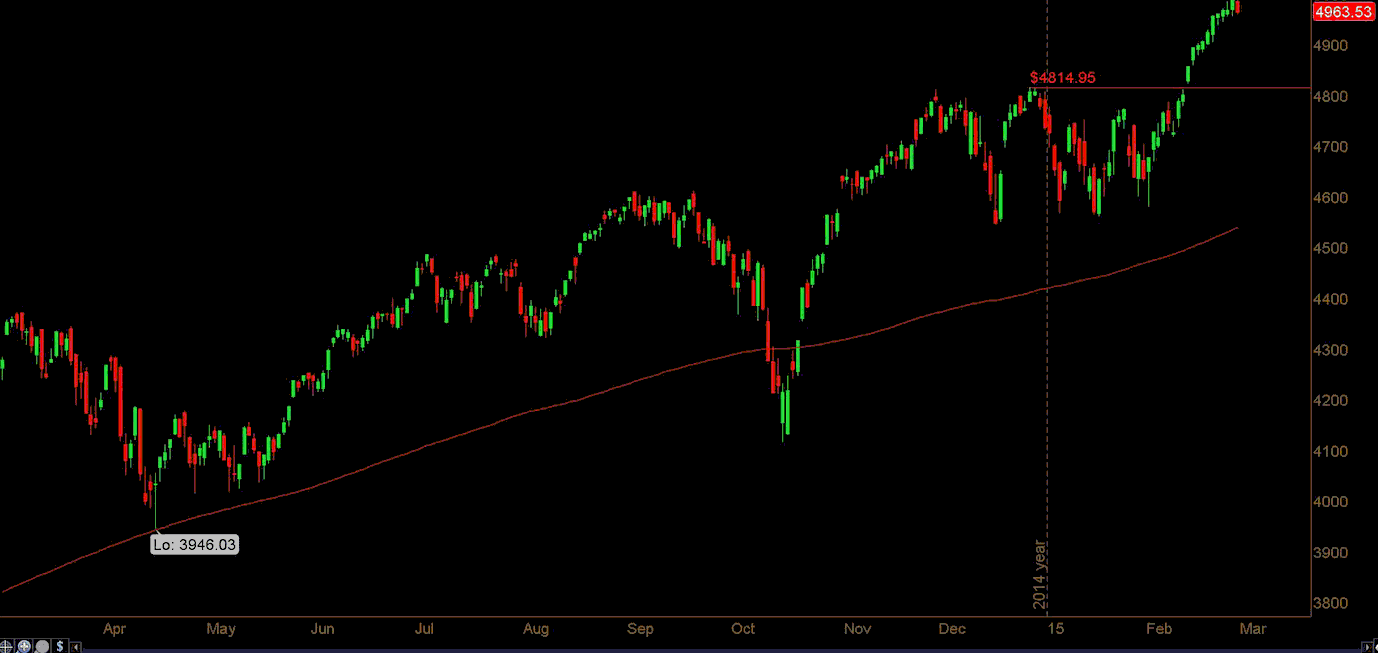
\includegraphics[scale=.3]{./images/stock.png}
		\end{center}
		\label{fig1}{Hình 3: Bảng dự đoán mức tăng trưởng của cổ phiếu (Hình minh họa)}
	\end{figure}
\end{center}


Nắm bắt được nhu cầu thực tế đó, người ta mới đưa, chỉnh sửa, phân tích các dữ liệu về thị trường, chính trị, xã hội sang dạng số liệu theo thời gian và áp dụng vào bài toán time series forecasting. Mặc dù vậy, có lẽ là do số liệu thu thập vẫn còn thiếu sót hoặc mô hình dự đoán vẫn chưa hoàn chỉnh nên kết quả dự đoán vẫn còn nhiều thiếu sót, không chiếm lấy được sự tin tưởng của người sử dụng. Tuy nhiên, các phương pháp mới vẫn được đang nghiên cứu sao cho kết quả ngày một chính xác hơn. Điều này mang đến một tương lai đầy hứa hẹn cho các nhà chơi cổ phiếu, và cũng có thể là thu hút thêm nhiều người chơi cổ phiếu hơn nữa do tính đơn giản mà nó mang lại.


\vspace{1cm}
\changefontsizes{15pt}
\setlength{\parindent}{0cm}
\textbf{Dự báo thời tiết}

\vspace{0.5cm}
\changefontsizes{13pt}
\setlength{\parindent}{0cm}

Dự báo thời tiết chính xác đem lại nhiều lợi ích cho không ít các ngành nghề, lĩnh vực trong xã hội. Theo phương pháp truyền thống, quá trình dự báo thời tiết thường trải qua các giai đoạn:  Quan trắc, trao đổi số liệu, phân tích, dự báo và phân phát sản phẩm dự báo. Với dữ liệu đã có, người ta sẽ phải thực hiện hàng tỉ phép tính trước khi cho ra dữ liệu cuối cùng, do đó vô cùng tiêu tốn thời gian và chi phí. Đây cũng là quy trình cơ bản của các loại hình dịch vụ dự báo thời tiết.



\begin{center}
	\begin{figure}[htp]
		\begin{center}
			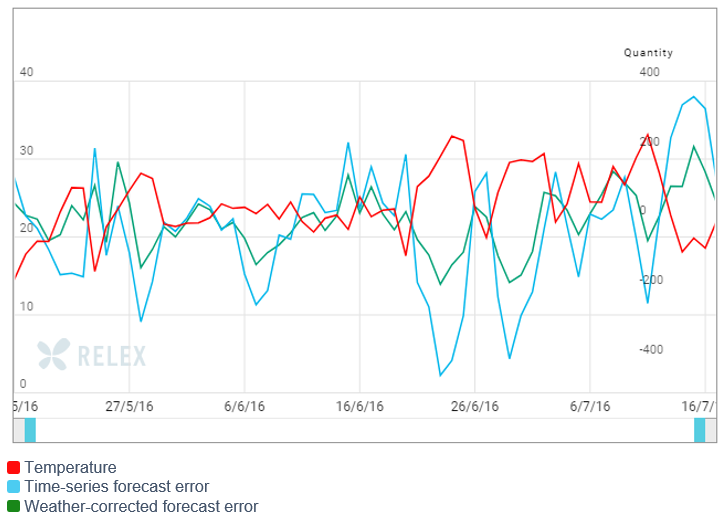
\includegraphics[scale=0.8]{./images/pre.png}
		\end{center}
		\label{fig1}{Hình 4: Bảng minh họa kết quả dự báo thời tiết (Hình minh họa)}
	\end{figure}
\end{center}


Với việc thu thập, ghi lại các thông tin về trạng thái của khí quyển, nhiệt độ, độ ẩm, gió,... theo các mốc thời gian cụ thể. Đã đem lại tính tương thích cao cho bài toán series forecasting. Và đúng như mong đợi, hiệu quả mà time series forecasting mang đến cho ngành dự báo thời tiết như một làn sóng mới về sự đơn giản, chính xác, tiết kiệm chi phí và nhanh chóng. 




\vspace{1cm}
\changefontsizes{15pt}
\setlength{\parindent}{0cm}
\textbf{Dự đoán doanh thu}

\vspace{0.5cm}
\changefontsizes{13pt}
\setlength{\parindent}{0cm}

Có thể nói việc tính toán doanh thu trong một sự kiện hoặc một giai đoạn thời gian sắp tới đối với các ngành nghề liên quan đến sản xuất, mua bán, dịch vụ,... là một trong những công việc đòi hỏi sự tỉ mỉ và khó khăn nhất. Bởi nó giúp nhà đầu tư biết rằng, liệu họ có nên đầu tư vào cái này thay vì cái kia không?, liệu họ có nên mở rộng cơ sở trong tháng sắp tới hay không? nếu mở thì nên mở thêm bao nhiêu cửa hàng? Tổng quát hơn, nó ảnh hưởng trực tiếp đến hành động và quyết định của nhà đầu tư, của người sở hữu cửa hàng, sở hữu doanh nghiệp,...


\begin{center}
	\begin{figure}[htp]
		\begin{center}
			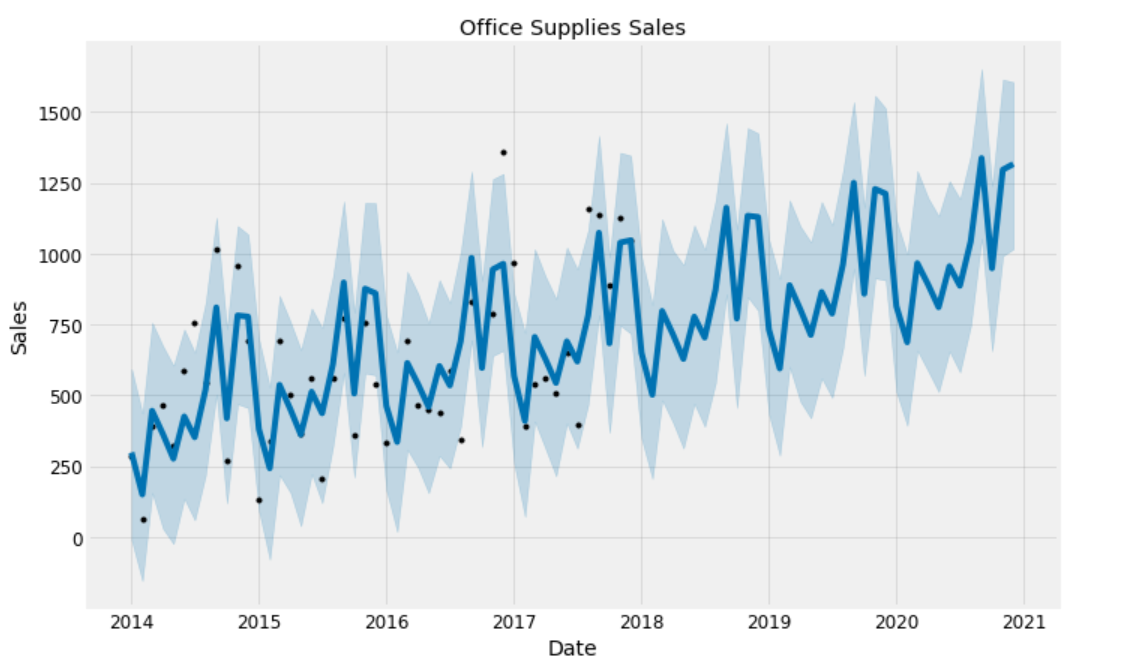
\includegraphics[scale=0.4]{./images/sales.png}
		\end{center}
		\label{fig1}{Hình 5: Bảng dự đoán hạn mức doanh thu theo từng năm (Hình minh họa)}
	\end{figure}
\end{center}


Từ ngàn xưa, từ trước khi người kinh doanh bắt đầu sử dụng máy tính để dự đoán mức doanh thu của mình, để tính toán mức doanh thu hì họ thường xem xét các vấn đề loại mặt hàng nào đang yêu thích? đang bán chạy? Có bao nhiêu cửa hàng đang kinh doanh loại mặt hàng này trong khu vực? Họ có bán chạy không? Vô số câu hỏi như thế sẽ được đặt ra, và sau khi trả lời tất thảy các câu hỏi đó, người ta sẽ dự đoán (phần lớn các trường hợp là ước lượng) mức doanh thu mà họ thu được nếu người ta đầu tư vào loại mặt hàng, lĩnh vực đó. Nghe có vẻ đơn giản, nhưng để tính toán tốt, ít sai sót nhất thì số câu hỏi đặt ra phải lên tới hàng trăm, có khi hàng nghìn câu hỏi, và với mỗi câu hỏi người ta phải có câu trả lời dưới dạng số liệu (dĩ nhiên số liệu này phải gần với thực tế nhất có thể). Tuy nhiên phương pháp vừa nêu chỉ dành cho những doanh nghiệp khổng lồ, đa phần các doanh nghiệp vừa và nhỏ chỉ xem xét và đặt ra một vài câu hỏi trọng yếu, do đó mà các kết quả thu được cũng khác nhau.

\bigskip
Cho đến khi người ta bắt đầu nghĩ đến việc dùng máy tính để thay mình tính toán doanh thu, họ cũng dùng các phương pháp, các công cụ công nghệ cao thay họ thu thập dữ liệu, sau đó sắp xếp thành các chuỗi dữ liệu theo thời gian. Vâng, rất phù hợp với bài toán time series forecasting. Tương tự như trên, time series forecasting cũng cho ra các kết quả dự đoán có độ chính xác đến bất ngờ (ở một vài trường hợp hầu như trùng khớp). Nhờ vào điều này, không chỉ có các công ty, doanh nghiệp lớn mới có thể đưa ra các quyết định đúng đắn, tầm cỡ, mà còn mở rộng cơ hội cho các doanh nghiệp, công ty nhỏ lẽ khác. Góp phần cho sự phát triển chung của toàn xã hội.

